\documentclass[12pt,twoside]{article}
\renewcommand{\abstractname}{\vspace{-\baselineskip}}
\usepackage{hyperref}
\usepackage{setspace}
\usepackage{indentfirst}
\urlstyle{same}
\usepackage{geometry}
 \geometry{left=1.25in, right= 1.25in ,top=1.7in}
\setlength{\parindent}{.5in}
\renewcommand{\baselinestretch}{1.3}
\setlength{\parskip}{\baselineskip}
\usepackage{xcolor}
\usepackage{fancyhdr}
\usepackage{caption}
\captionsetup{font={normalsize,stretch=1}}
\renewcommand{\headrulewidth}{0pt}
\usepackage[labelfont=bf]{caption}
\captionsetup[figure]{labelfont={bf},name={Figure},labelsep=period}
\usepackage{natbib}
\setlength{\bibhang}{0.5in}
\bibliographystyle{apalike}
\usepackage{graphicx}
\usepackage{float}
%\usepackage{floatrow}
%  \floatsetup[table]{capposition=top}
\usepackage{booktabs}
\usepackage{tabularx}
\usepackage{titling}
\settowidth{\thanksmarkwidth}{*}
\setlength{\thanksmargin}{-\thanksmarkwidth}
\usepackage[hang,flushmargin]{footmisc}
\setlength{\skip\footins}{1.2pc plus 5pt minus 2pt}
\usepackage{titlesec}
\setlength{\droptitle}{-5em}
\setlength\thanksmarkwidth{.5em}
\setlength\thanksmargin{-\thanksmarkwidth}
\titleformat{\section}{\normalfont\bfseries\filcenter}{}{0pt}{}
\titleformat{\subsection}{\normalfont\bfseries\filcenter}{}{0pt}{\itshape}
\titleformat{\subsubsection}{\normalfont\bfseries\filcenter}{}{0pt}{\itshape}
\titlespacing*{\section}
  {0pt}{-.1\baselineskip}{-.1\baselineskip}  
\titlespacing*{\subsection}
   {0pt}{-.1\baselineskip}{-.1\baselineskip}  
\usepackage[T1]{fontenc}
\usepackage{fontspec}
  \fontspec{Times New Roman}
\date{}
\providecommand{\keywords}[1]
{
   \small	
  \textit{\hspace{-1em} Keywords: } #1
}
%\newfontfamily\headingfont[]{Times New Roman}
%Add Author names to headers and footers here:
\fancypagestyle{firstpage}{
  \fancyhf{}% clear all fields
  \fancyfoot[L]{ \footnotesize Copyright \copyright 2021 (Luehring et al.). Creative Commons Attribution-NonCommercial-NoDerivatives 4.0 International Public License. Available at: \url{http://journalqd.org}} 
  \lhead{ \footnotesize Journal of Quantitative Description: Digital Media 1(2021), 1–n} %Replace n with number of last page, including the Online Appendix.
\rhead{ \footnotesize 10.51685/jqd.2021.XXX}
}
\pagestyle{fancy}
\fancyhf{}
\fancyhead[LO]{ \footnotesize Journal of Quantitative Description: Digital Media 1(2021)}
\fancyhead[RO]{ \footnotesize Reviewing NewsGuard \thepage} %Select Short Title with fewer than 35 characters.
\fancyhead[LE]{ \footnotesize Luehring et al.} %(Author1 & Author2) or (Author1 et al.)
\fancyhead[RE]{ \footnotesize Journal of Quantitative Description: Digital Media 1(2021) \thepage}

%Article Title
\title{ \normalsize \textbf{} \vspace{-1.5em} Reviewing domain-based approaches to track untrustworthy domains: How reliable is the NewsGuard database?}
%Author names and affiliations go here in the single \author{} , put authors' contact information in \thanks{}. Use extra spacing: \vspace{1em} to separate authors (unless the authors share the same affiliation.  
\author{\normalsize LUEHRING, JULA \\ \normalsize University of Vienna \& Complexity Science Hub, Vienna, Austria 
\vspace{1em} \\ \normalsize LAZZARONI, RUGGERO MARINO \\ \normalsize RWTH Aachen, Germany \vspace{1em} \\ \normalsize LASSER, JANA \\ \normalsize TU Graz, Austria \thanks{\hspace{-1em} Author 1: jula.luehring@univie.ac.at} \thanks{\hspace{-1em} Author 2: author2's email address} \thanks{\hspace{-1em} Date submitted: XXXX-XX-XX}} 

\renewcommand\footnotemark{}
\begin{document}
\maketitle
\thispagestyle{firstpage}
\vspace{-8em}
\begin{abstract}
\noindent To study the spread of misinformation on digital platforms, it is imperative for computational social scientists to have access to reliable and valid tools that enable them to identify misinformation. A prominent way to track misinformation is to use a list of domains. For example, the organization NewsGuard offers the most comprehensive database of domain trustworthiness ratings and is increasing in popularity. Despite restrictive access, the database was never created as a research instrument and has never been reviewed systematically.
\end{abstract}
\keywords{\textit{misinformation, NewsGuard, social media} \vspace{8ex}}

\section{Introduction}
%% MISINFORMATION.
Misinformation is widely visible on social media \citep{lazerScienceFakeNews2018} and in the mainstream media \citep{tsfatiCausesConsequencesMainstream2020}. However, only a small number of people engage with unreliable information online~\citep{allenEvaluatingFakeNews2020, grinbergFakeNewsTwitter2019}. Typically, these people are strong partisans (REF). Misinformation seems to feed into growing partisan sorting and intergroup animosity~\citep{gonzalez-bailonAsymmetricIdeologicalSegregation2023a, robertsonUsersChooseEngage2023a}, exploiting the dynamics at play by fueling conflict and negative emotions. Consequently, it is imperative to understand the spread of misinformation and its interactions with digital media. In order to do so, computational social scientists require access to reliable and valid data. 

The spread of misinformation has been studied extensively by scholars from various scientific disciplines, therefore, relying on diverse conceptualizations. Definitions of misinformation seem to largely depend on the respective methodological choices, resulting in imprecise or inconclusive findings \citep{altayMisinformationMisinformationConceptual2023a}. To study the diffusion or discussion of misinformation on social media, computational researchers commonly follow a selection of stories or sources. Both approaches typically rely on experts, such as fact-checkers, to curate a list that is then used as a starting point to collect data from one or more digital platforms. The choice between story and source-based approaches hinges on the primary research objective: When operating at the level of the story, we capture misinformation with high precision, but the selection of stories can be narrow and is likely biased. Conversely, with a source-based strategy, we can cover a wider variety of sources and stories, and hence, the data may be less biased. However, the latter, source-based approach runs the risk of overgeneralizing across stories, and source ratings may be especially sensitive to time and context. 

%% NEWSGUARD.
A prominent way to track misinformation is to use a list of untrustworthy domains. The organization \href{https://www.newsguardtech.com/}{NewsGuard} offers the most comprehensive database, not just blacklisting domains but providing a trustworthiness score per domain. A team of journalists and editors rate the domains based on nine journalistic quality criteria and regularly updates both the coverage of the list, i.e., the number of domains, as well as their overall trustworthiness rating. Recently, the database has been extended to other countries than the United States and is constantly growing. Despite increasing popularity~\citep[for example,][]{robertsonUsersChooseEngage2023a,lasserSocialMediaSharing2022a}, however, the database was created as a tool for brand security rather than research, which is why access is not public and expensive. Consequently, we provide a comprehensive description of the content of this database and introduce our research question: How reliable is the NewsGuard database of domain trustworthiness ratings over time and language contexts?

More precisely, we believe that it is essential to address the following aspects of the database in more detail: the distribution, construction, weighting and update process of the ratings, the selection and removal of domains, and the completeness and reliability of other information provided in the database, e.g., political orientation. Therefore, we focus on three questions:
\begin{itemize}
    \item \textbf{How volatile are trustworthiness ratings, e.g., how often do ratings change or domains vanish?} This is important to estimate whether using an older database will distort results. We reproduce published research relying on the NewsGuard list with different versions of the list to assess the degree to which results depend on a specific version of the list.
    \item \textbf{How reliable and complete is the provided information, particularly for non-US countries?} A recent study has shown high agreement of NewsGuard with other expert-rated lists in the U.S. context~\citep{linHighLevelCorrespondence2023}, but an assessment for other countries and contexts is missing. 
    \item \textbf{How can other information be used for misinformation research?} For each domain, NewsGuard experts rate journalistic quality criteria, topics, and political orientation, but they also label AI-generated content. Estimating to what extent the different criteria constitute the overall trustworthiness score and the completeness of additional information might shed light on aspects of misinformation beyond binary true/false labels.
\end{itemize}
By describing the database, we outline potential pitfalls for digital media research and offer recommendations for the application of the NewsGuard database in different contexta. We also want to empower misinformation researchers to make informed decisions about whether the substantial expense associated with acquiring access to NewsGuard is necessary for their research. 

\section{Results}
As of September 20, 2023, the database contains 11,093 trustworthiness assessments. For every domain, this includes (see Table for full list of variables):
\begin{itemize}
    \item Domain and trustworthiness rating (between 0 and 100).
    \item Binary labels for nine journalistic quality criteria constituting the trustworthiness rating. 
    \item Language and country associated with the domain.
    \item Political orientation of the outlet.
    \item Topics covered (e.g., ``local news'', ``political news'', ``health information'') by the outlet
    \item A flag indicating whether the outlet frequently posts AI-generated content.
    \item 
\end{itemize}

\subsection{How volatile are trustworthiness ratings?}
A trained team of NewsGuard experts regularly assesses the trustworthiness of selected news outlets. However, the organization also manually adds outlets they deem influential or that changed domains. The organization saves hourly snapshots of the database, allowing us to track changes going back to March 2019, when the organization started operating. Here, we review the distribution, construction, weighting and update process of the ratings over the years. 

%%distribution
NewsGuard trustworthiness ratings are assigned on a scale from 0 to 100, with 100 being trustworthy. The threshold for the trustworthiness of a source is set at 60. Notably, NewsGuard is not a blacklist. In fact, close to 60\% of domains have an overall rating of over 60 and are therefore considered ``trustworthy''(see Fig.~\ref{fig:fig1}) for the distribution of trustworthiness scores. 
\begin{figure}[!ht]
    \centering
    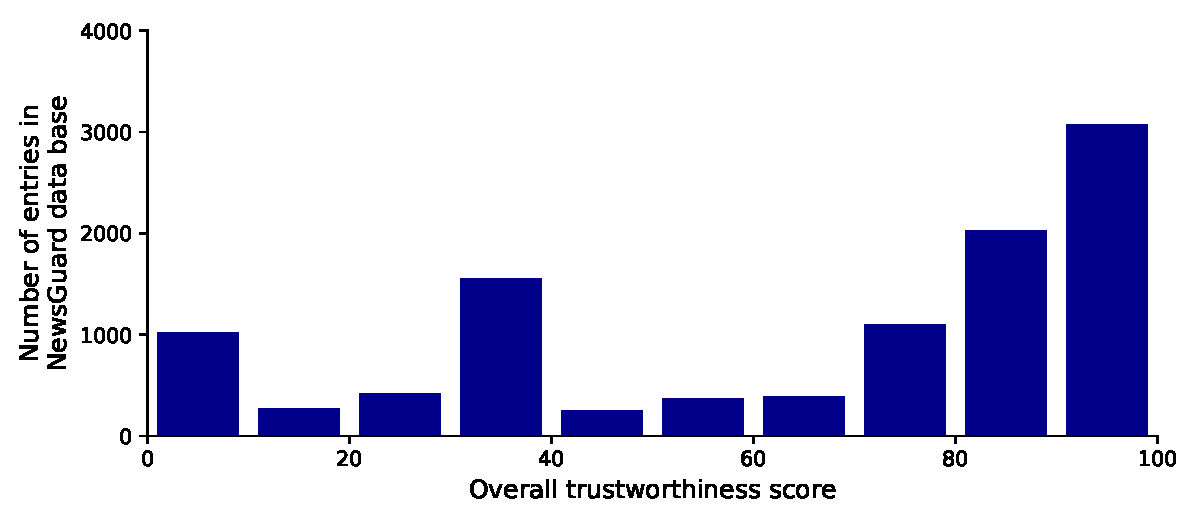
\includegraphics[width=\textwidth]{NewsGuard_histogram.pdf}
    \caption{Distribution of domain trustworthiness contained in the NewsGuard database as of September 20, 2023.}
    \label{fig:fig1}
\end{figure}

In addition, some sources do not receive a trustworthiness score as they are classified as a ``platform'' (420 domains, e.g., Facebook, Twitter, YouTube). In addition, the database includes 387 sources judged as ``satire'' (e.g., The Onion, The Babylon Bee). Both platforms and satire sources are not rated by NewsGuard, but they are included in the database. We exclude them from our further analyses. 

%%development over time
When looking at the score distribution over time, the right skew has been diminishing; while the mean and median rating averaged per year, was XY in 2019, it is now XY. In other words, the average trustworthiness of domains has increased over time. The distributions of trustworthiness over time are shown in Figure XY.

%%added vs updated sources
However, new sources added to the database tend to have a lower score, as shown in Figure XY. This is likely due to the fact that the organization has been adding untrustworthy domains. A great number of sources have been added in September 2020, which might explain the lower average trustworthiness score in the following. In contrast, scores of already covered sources tend to decrease over time, i.e., when NewsGuard updates trustworthiness ratings, they tend to get a lower score. This is shown in Figure XY. 

%%construction
The trustworthiness score is a composite score that calculated based on nine journalistic criteria. For each domain, the organization assigns a binary label (yes/no) per criterion. The trustworthiness score is then calculated as the sum of the weighted criteria. 
The criteria are weighted differently, ordered in descending relevance:
\begin{itemize}
  \item ``Does not repeatedly publish false content'' (22 points)
  \item ``Gathers and presents information responsibly'' (18 points) 
  \item ``Regularly corrects or clarifies errors'' (12.5 points)
  \item ``Handles the difference between news and opinion responsibly'' (12.5 points)
  \item ``Avoids deceptive headlines'' (10 points)
  \item ``Website discloses ownership and financing' (7.5 points)
  \item ``Clearly labels advertising'' (7.5 points)
  \item ``Reveals who's in charge, including possible conflicts of interest'' (5 points)
  \item ``The site provides the names of content creators, along with either contact or biographical information'' (5 points)
\end{itemize}

Further explanation of the criteria and their weights can be found in the NewsGuard FAQ\footnote{\href{https://www.newsguardtech.com/ratings/rating-process-criteria/}{https://www.newsguardtech.com/ratings/rating-process-criteria/}}. 

In the latest version of the dataset, the first criterion was the most respected and XY of sources satisfy it. Across all versions of the dataset, the most common combination of values is that all criteria are satisfied (XY\% of sources), given that most sources are considered trustworthy. The second most common combination is that all criteria are satisfied except for the criterion ``Does not repeatedly publish false content'' (XY\% of sources).

Furthermore, looking at domain criteria updates, we find that most sources also keep their scores. However, the most common update pattern is a negative change in the criterion ``Website discloses ownership and financing'', occurring for sources like XYZ. This criterion appears to be the most volatile, with XY\% of sources changing their label for this criterion. On the other hand, a positive update is also the fourth most common pattern, showing that it might be the one that is most frequently updated/monitored by NewsGuard.

\subsection{How reliable and complete is the provided information, particularly for non-US countries?}
Over the span of four years, NewsGuard has grown from 2,641 to 9,734 domains, as shown in Figure X. The selection and removal of domains is unclear. Still, the organization claims to have reviewed domains accounting for 95\% of online engagement.
\begin{figure}[!ht]
    \centering
    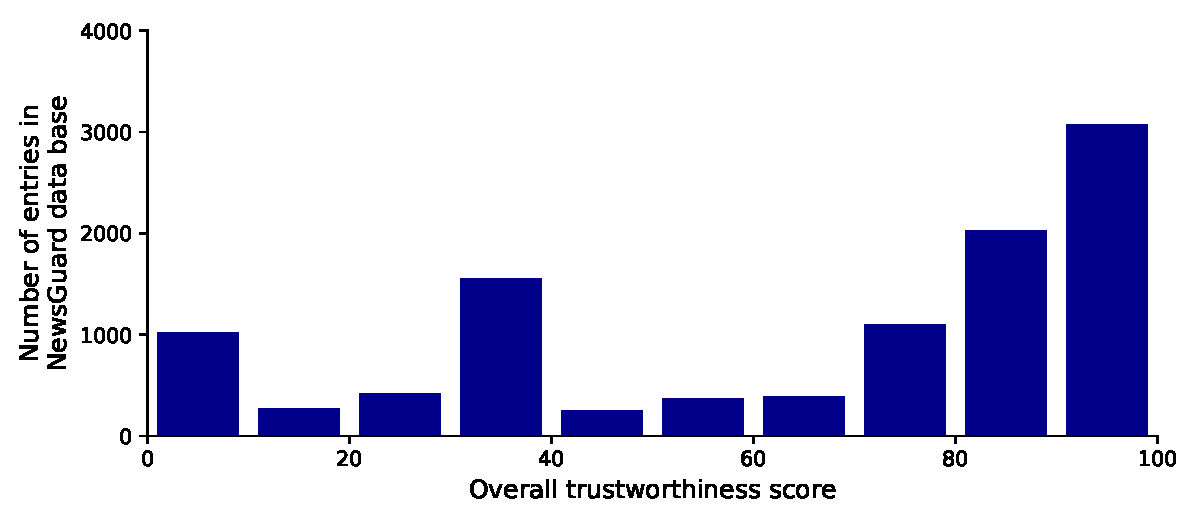
\includegraphics[width=\textwidth]{NewsGuard_histogram.pdf}
    \caption{Distribution of domain trustworthiness contained in the NewsGuard database as of September 20, 2023.}
    \label{fig:fig2}
\end{figure}

The dataset contains sources for nine countries in total (United States, Italy, Great Britain, France, Germany, Canada, Australia, Austria, New Zealand) plus sources considered to be global. The majority of sources are from the United States (66\%), followed by global sources (12\%), Great Britain (5\%), Italy (5\%), Canada (4\%), France (4\%) and Germany (3\%). The remaining countries account for less than 1\% of sources each. The dataset also clusters sources based on language (English, Italian, French, German, Spanish). See Table X for an overview of the number of sources per country and language, as well as distribution of scores, topics, and political orientation.

%%completeness
In latest iteration, sources have a mean rating of 64.49, a median of 77.5 (SD = 32.56). The statistics appear to be uniform, except for US sources: U.S.-based outlets are of lower quality on average, which could be related to the relative number of outlets in the dataset (6433 US sources versus 375 sources per other countries on average).

%%reliability

\subsection{How can other information be used for misinformation research?}
\textbf{Political Orientation}
The dataset also classifies sources according to their political orientation. The classification relies on a left-to-right conception of the political spectrum and should be interpreted in the context of the respective political landscape. Over the years, the labels have shifted from four to only two possible labels (left/right). 

%%completeness
Overall, the political orientation dimension covers only a minority of the sources in the database. Out of 9,811, 3,343 sources have a political orientation rating. The ratio decreases when zooming in on singular countries: only 42.87\% of news outlets have a political orientation rating in the United Stated, 14.57\% in Great Britain, 16.49\% in Italy, 19.74\% in Germany, 4.92\% in Canada, and 10\% in New Zealand. Here, again the United States is overrepresented in the dataset.

%%distributions 
Trustworthiness ratings are lower for right-leaning sources. The mean trustworthiness score for right-leaning sources is 58.5, while it is 66.5 for left-leaning sources. The median is 65 for right-leaning sources and 77.5 for left-leaning sources. The distribution of scores is shown in Figure X.

\textbf{Topics}
The database assigns topic labels, which are based on the topics covered by the outlets. The topics are not mutually exclusive, i.e., a source can be assigned to multiple topics. The topics are, for instance, ``Local News'', ``Political News or Commentary'', or ``Conspiracy Theories or Hoaxes''.
The topics are also not exhaustive, as 1,366 sources are not classified under any topic (see Table for topic occurence). 

Trustworthiness ratings greatly differ across topics. Figure X shows that sources covering conspiracies have the lowest average rating, while those covering ``Technology'' (M=87.16) and ``Business or Personal Finance'' (M=83.21) have the highest average ratings. The category ``Political News and Commentary'' attracts the highes share of bad sources: 80.09\% of all untrustworthy sources are said to cover that topic, making up the 76\% of all sources covering that topic.

The ``Conspiracy'' label contains only 39\% of the untrustworthy sources, suggesting that it only makes up a small proportion of all untrustworthy information. Nonetheless, it is a highly typical topics for bad sources: 99\% of the sources connected to this topic are untrustworthy. the quality of sources linked to each topic is illustrated in Figure X. 

\textbf{AI-labelled content}

\section{Discussion}
Points:
Right-skewed distribution of scores reflects the presence of misinformation. Even if there are more sources out there, their prevalence should be small
Misses user-created misinformation

\section{Methods}

\section{Acknowledgments}
Acknowledgements/ Author's disclosure/ funding statement.

\bibliography{newsguard-review.bib}

\appendix
\section{Online Appendix}
Appendix goes here.
\end{document}